\apendice{Especificación de diseño}

\section{Introducción}
En este apartado se va a explicar el análisis y diseño de los datos. También se va a exponer cómo se han resuelto las especificaciones y los casos de uso mencionados en el apartado anterior.  

Uno de los objetivos de este apartado es la comprensión  de la toma de decisiones y los motivos o causas que han dado lugar a las mismas.

\section{Diseño de datos}


\subsection{Modelo Entidad-Relación(ER)}
A continuación en la figura \ref{fig:ModeloER} se observa el modelo ER o Diagrama Relacional de la Base de Datos de la aplicación.


\begin{figure}%[!h]
		\centering
		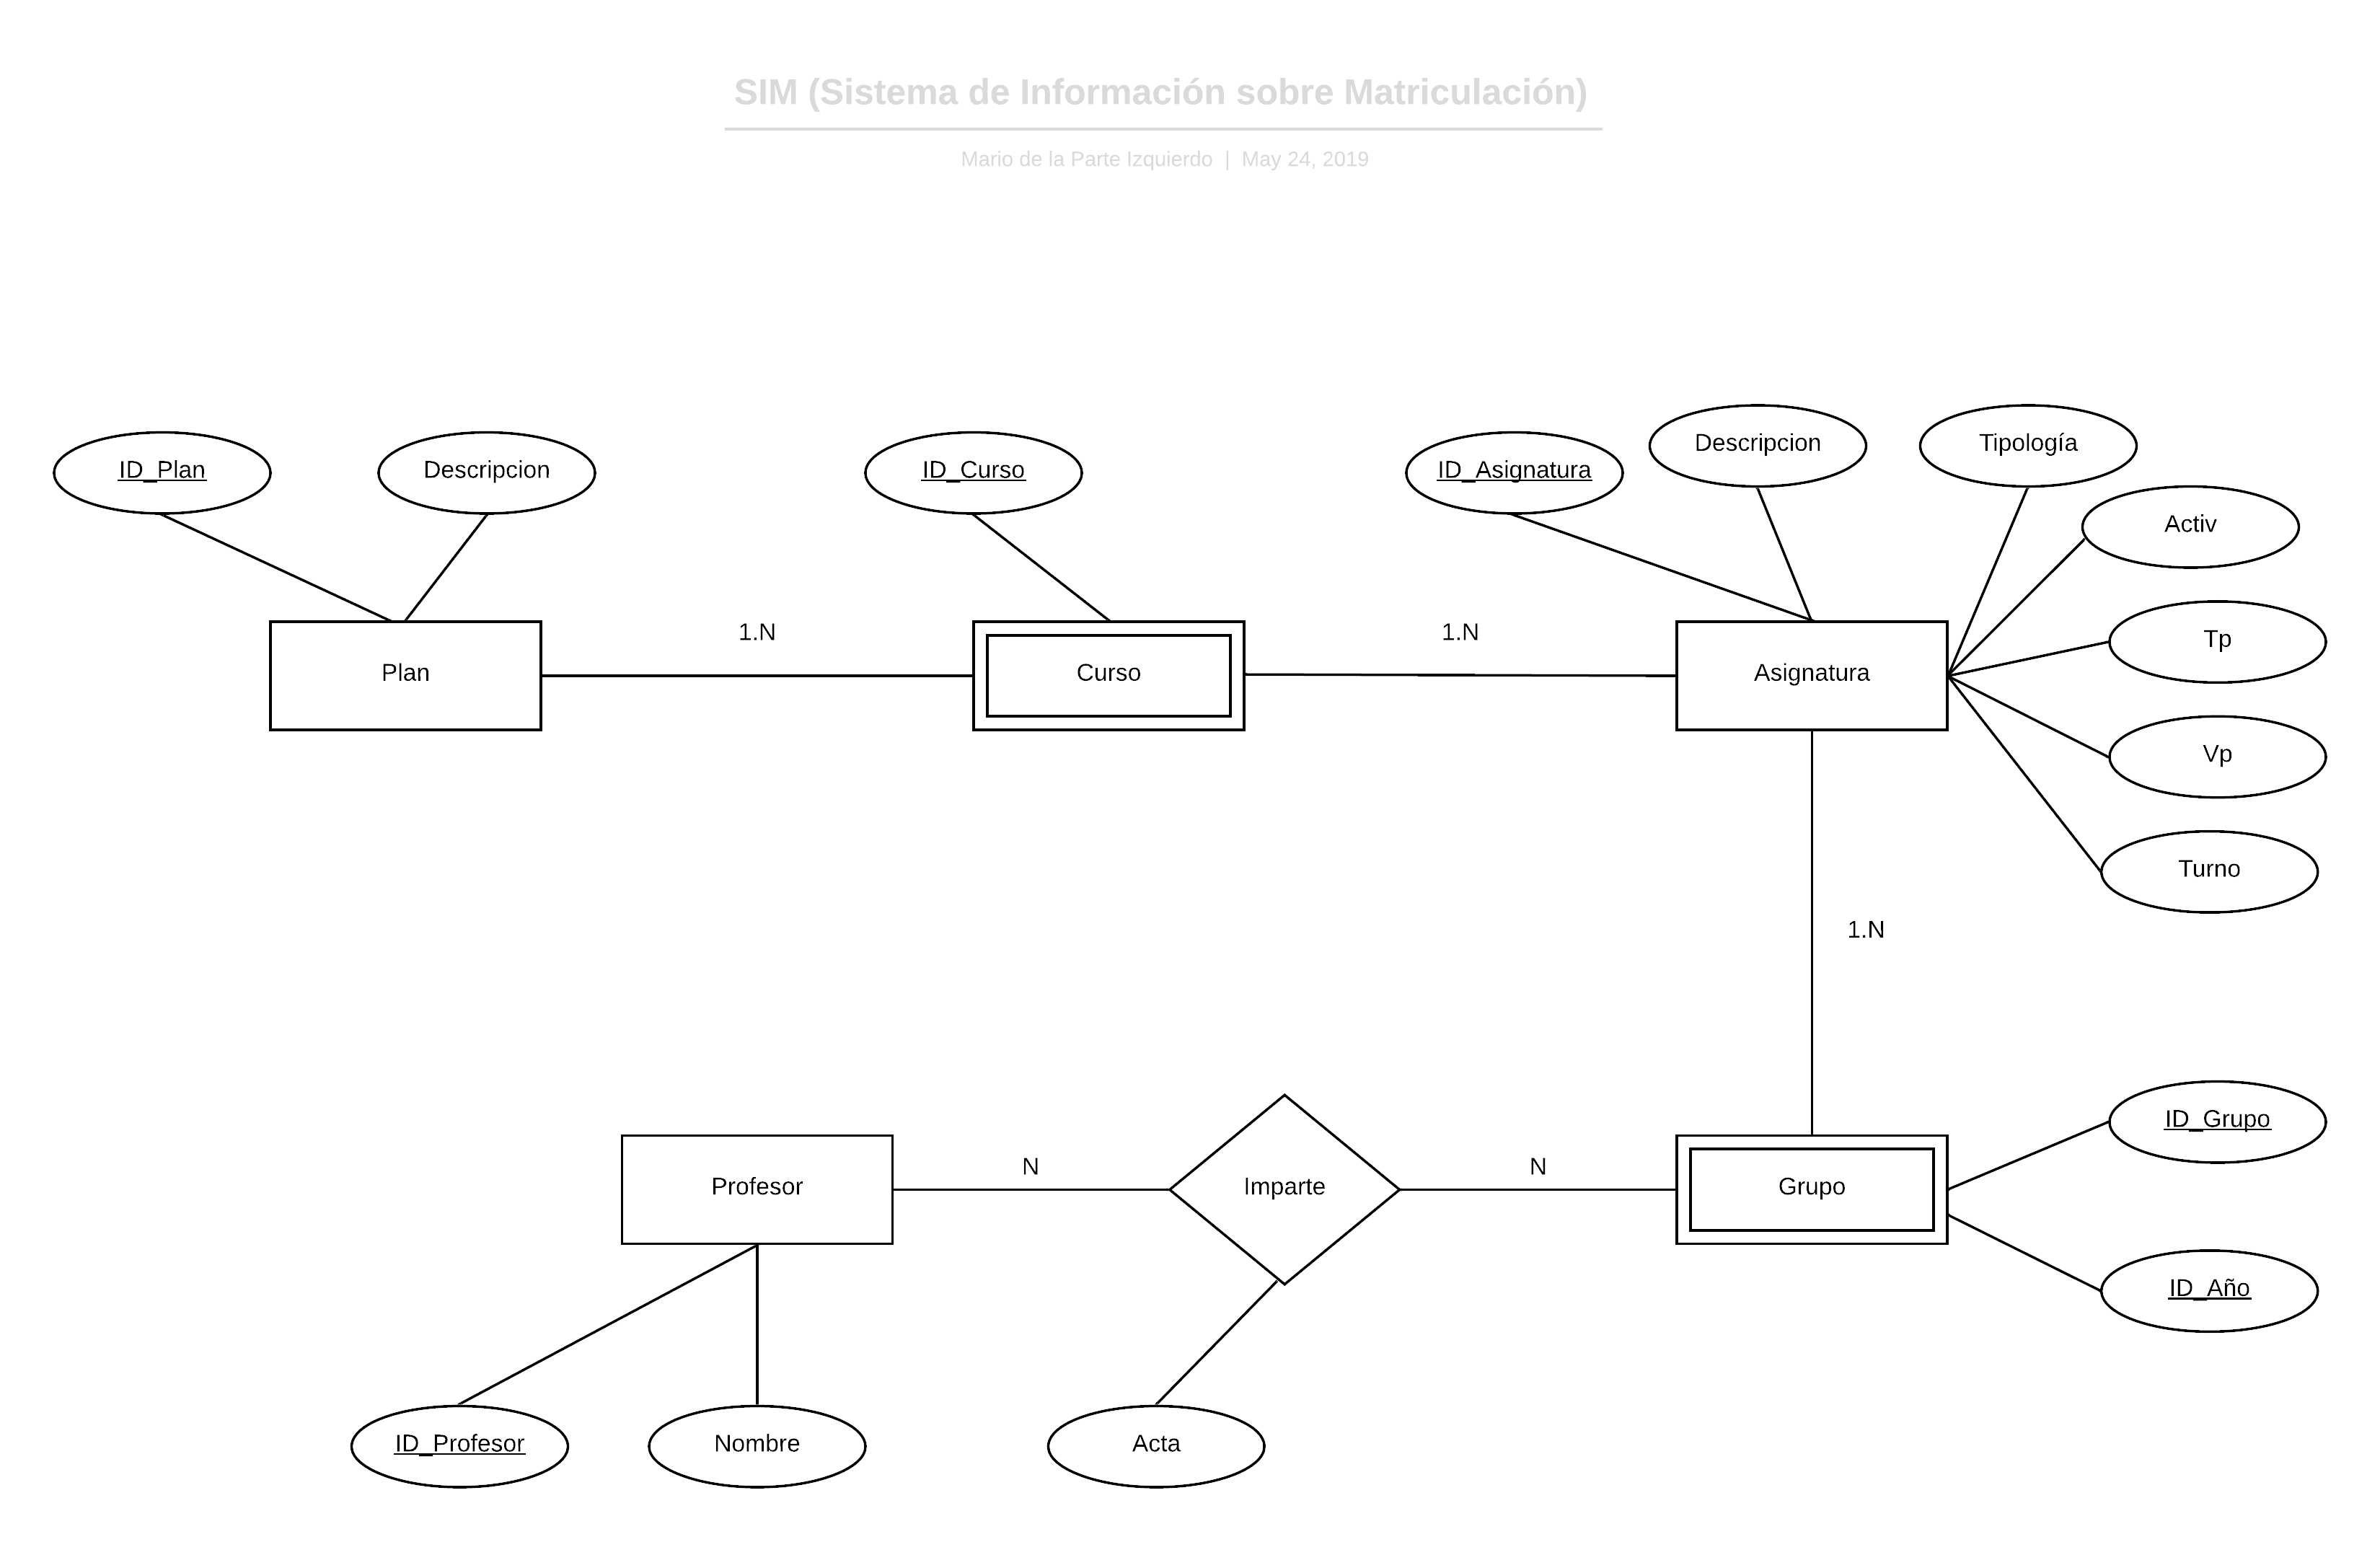
\includegraphics[angle=90, width=0.9\textwidth]{ModeloER}
		\caption{Modelo Entidad-Relación(ER)}\label{fig:ModeloER}
	\end{figure}

% \imagen{ModeloER}{Modelo Entidad-Relación(ER)}
%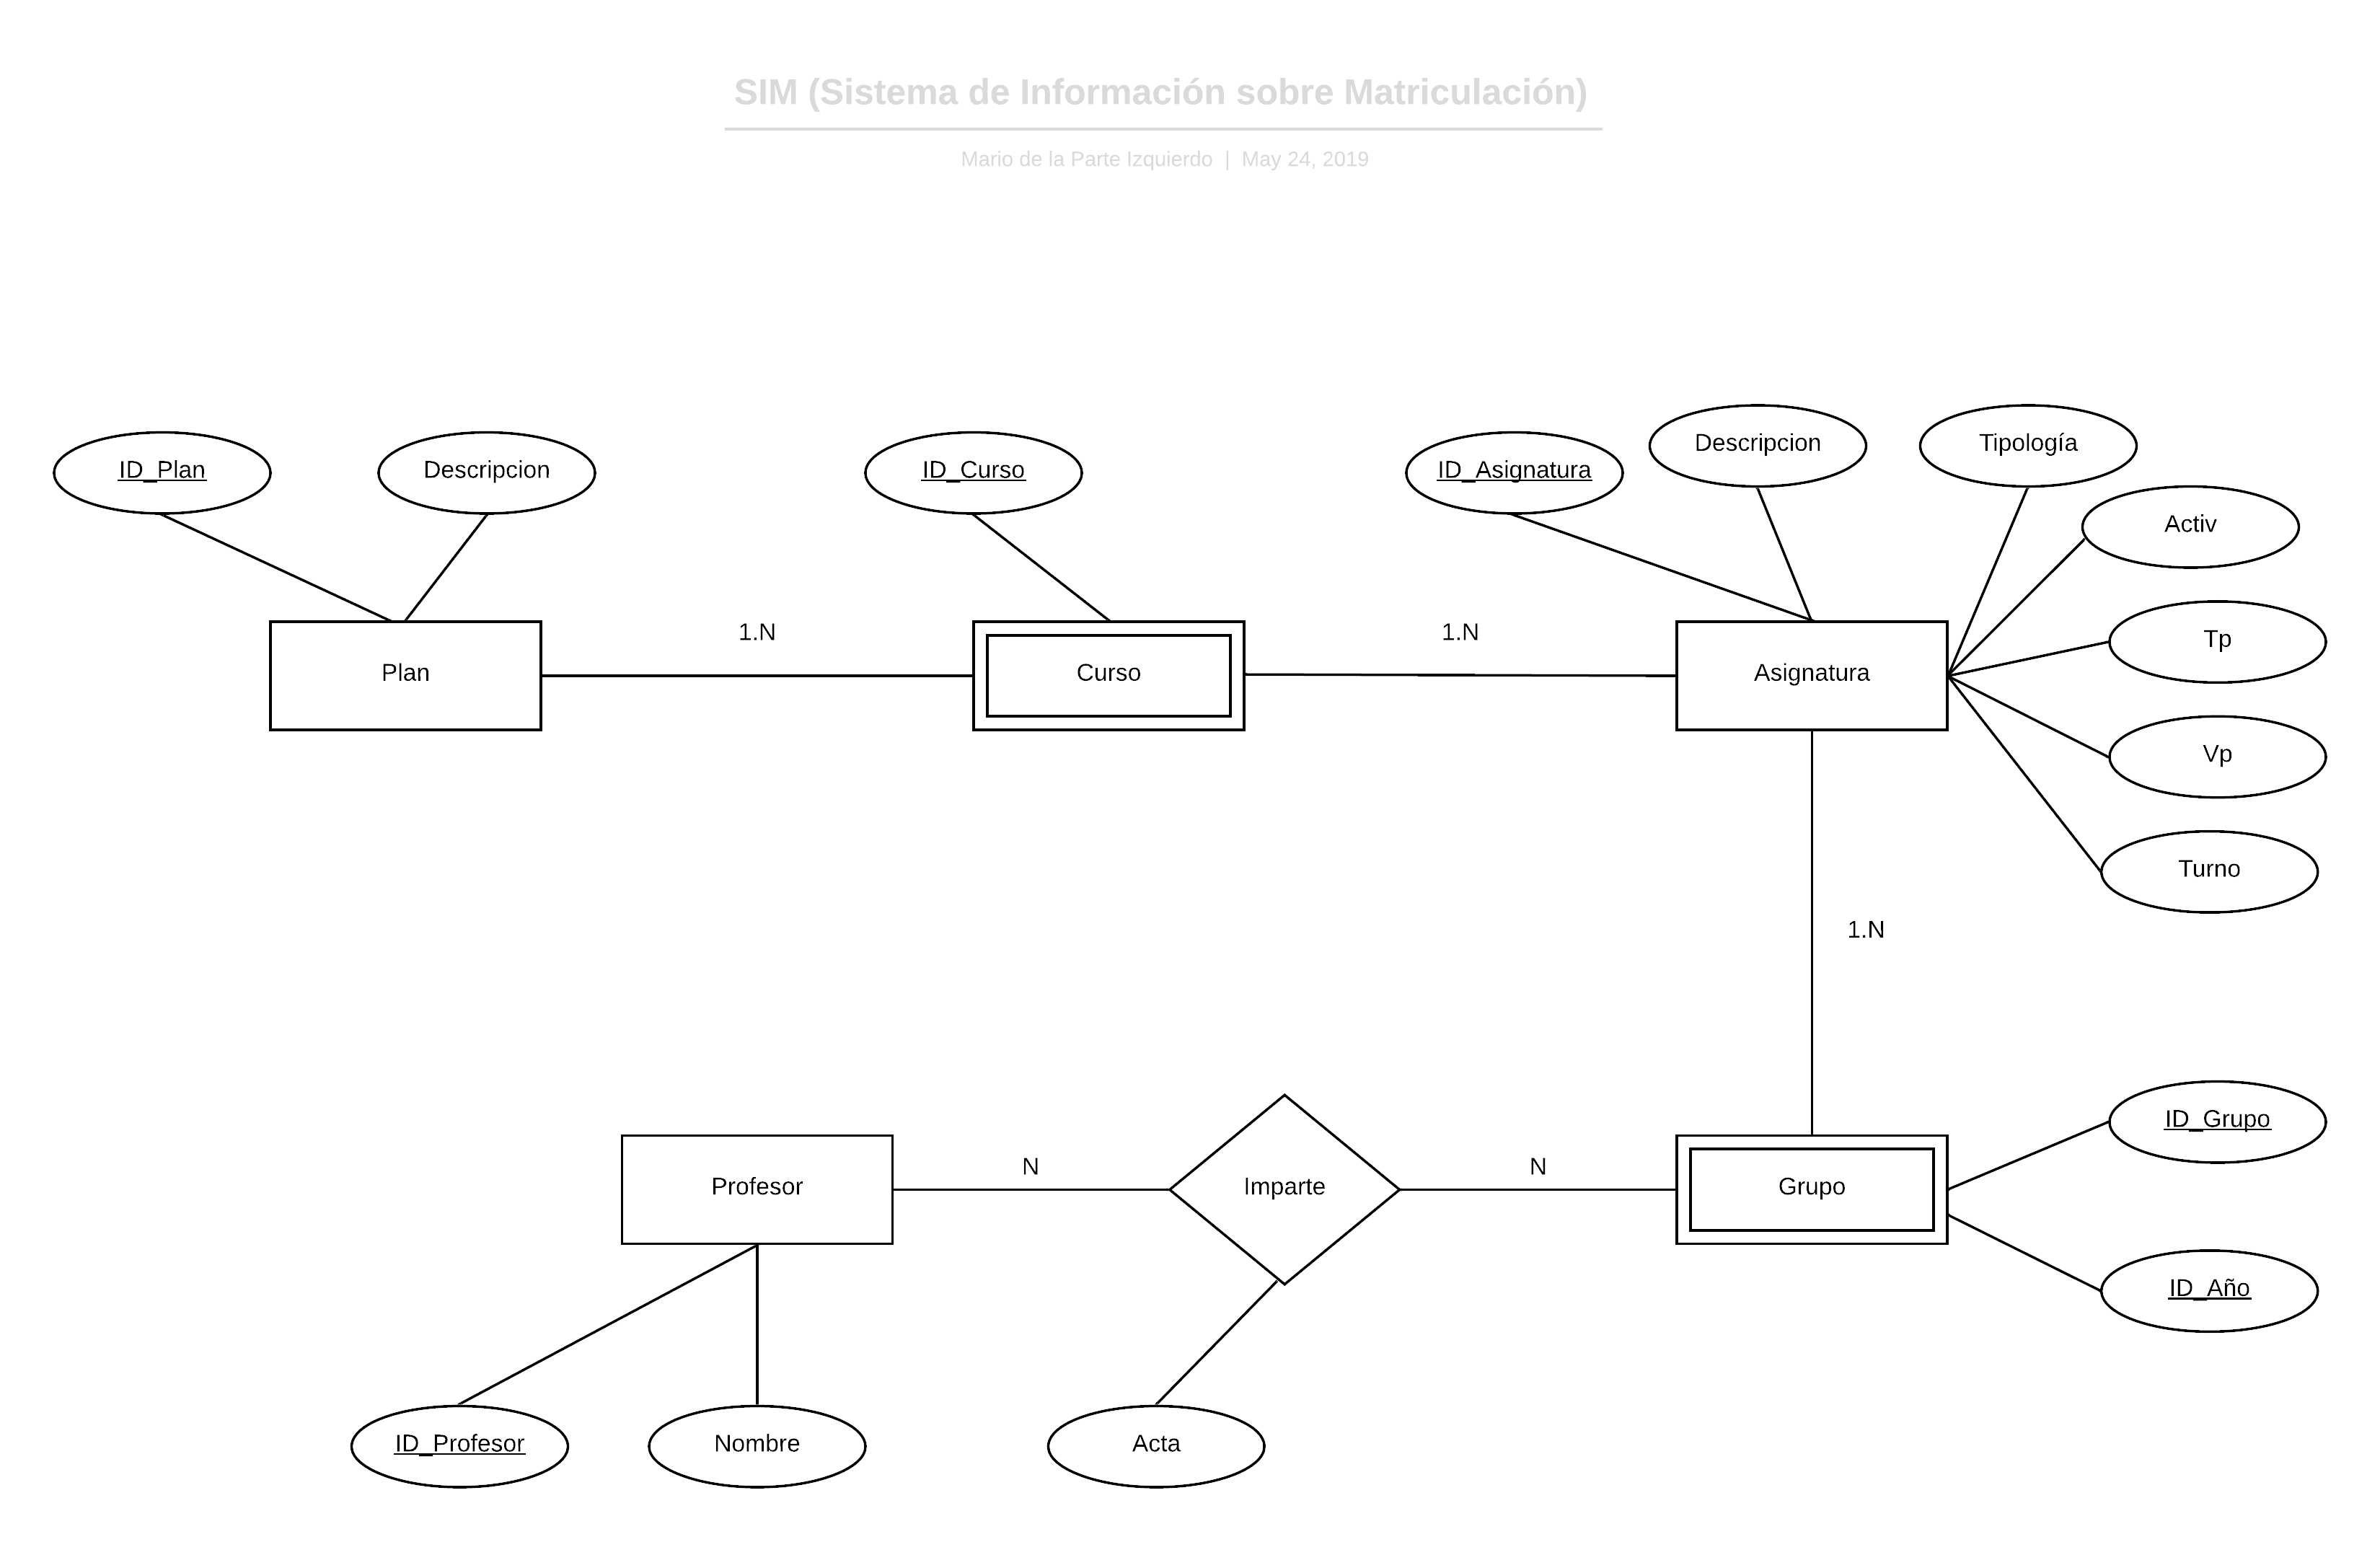
\includegraphics[angle=90, scale = 0.19]{ModeloER}

Se aprecia un total de cinco entidades, dos de las cuales son entidades débiles(\emph{Curso} y \emph{Grupo}). En las relaciones entre entidades se aprecia la cardinalidad entre las mismas, existiendo tres relaciones \emph{1.N} y una relación \emph{N.N} entre \emph{Profesores} y \emph{Grupo}. En cada entidad podemos apreciar sus atributos, así como sus claves primarias(subrayadas).



\subsection{Base de datos}
Se utiliza una base de datos(BBDD) para almacenar toda la información de la aplicación. La BBDD está compuesta por tres tablas principales:


\imagen{TablaASIGNATURAS}{Tabla ASIGNATURAS}

\begin{itemize}
\item
\textbf{ASIGNATURAS}: en esta tabla se almacena la información relacionada con las asignaturas que componen un Plan de Estudios o Titulación determinada. Esta tabla está formada por 9 campos, que son los siguientes:
\begin{itemize}
\item
\textbf{Id\_Asignatura}: es la clave primaria de la tabla y almacena el identificador único de la asignatura. Es un campo numérico de 4 dígitos.
\item
\textbf{Descripcion}: se almacena el nombre de la asignatura. Es un campo de caracteres.
\item
\textbf{Curso}: se almacena el curso al que pertenece la asignatura. Es un campo numérico de 1 dígito.
\item
\textbf{Plan}: se almacena el Plan de Estudios o Titulación al que pertenece la asignatura. Es un campo alfanumérico.
\item
\textbf{Tipologia}: se almacena la tipología del grupo, que puede ser teórica o práctica. Es un campo de caracteres.
\item
\textbf{Activ}: se trata de un campo de caracteres.
\item
\textbf{Tp}: se almacena el semestre académico. Es un campo de caracteres.
\item
\textbf{Vp}: es un campo numérico de 1 dígito.
\item
\textbf{Turno}: indica si el horario es de mañana, de tarde o mezcla de ambos(mixto). Se trata de un campo de caracteres.
\end{itemize}





\imagen{TablaGRUPOS}{Tabla GRUPOS}

\item
\textbf{GRUPOS}: en esta tabla se almacena la información relacionada con los grupos. Hay que destacar que esta tabla se trata de una entidad débil, como se ha visto anteriormente en el modelo de Entidad Relación(ER). Tiene una clave primaria formada por 3 capos (Id\_Asignatura, Id\_Grupo y Temporada(Año)) para poder identificar el total de alumnos matriculados en un grupo de una asignatura, en un año académico en concreto. Esta tabla, por lo tanto, está formada por 4 campos:
\begin{itemize}
\item
\textbf{Id\_Asignatura}: es la clave primaria de la tabla \emph{ASIGNATURAS} y almacena el identificador único de la asignatura. Es un campo numérico de 4 dígitos. Como se ha comentado, es un campo que forma parte de la clave primaria de \emph{GRUPOS}, junto a  Id\_Grupo y Temporada.
\item
\textbf{Id\_Grupo}: es el identificador de grupo y forma parte de la clave primaria junto a  Id\_Asignatura y Temporada. Es un campo numérico de 2 dígitos.
\item
\textbf{Temporada}: indica el año que se cursó o se va a cursar un grupo de una asignatura en concreto y por lo tanto, forma parte de la clave primaria junto a  Id\_Asignatura e Id\_Grupo. Es un campo alfanumérico.
\item
\textbf{Total\_Alumnos}: en este campo se almacena la cantidad de alumnos que hay matriculados en un grupo de una asignatura en un año determinado. Se trata, por tanto, de un campo numérico.
\end{itemize}




\imagen{TablaPROFESORES}{Tabla PROFESORES}

\item
\textbf{PROFESORES}: esta tabla surge de la relación entre las entidades \emph{Grupos}(entidad débil) y \emph{Profesores} como se ha apreciado anteriormente en el modelo Entidad Relación(ER). En esta tabla se almacena la información relacionada con los profesores y los grupos de asignaturas que imparten clase en un año determinado. Tiene una clave primaria formada por 4 campos (Id\_Profesor, Id\_Asignatura, Id\_Grupo y Temporada(Año)). Esta tabla, está formada por estos 6 campos:
\begin{itemize}
\item
\textbf{Id\_Profesor}: forma parte de la clave primaria de la tabla y almacena el identificador único de profesores. Es un campo numérico de 4 dígitos.
\item
\textbf{Id\_Asignatura}: es un campo que forma parte de la clave primaria y almacena el identificador único de la asignatura. Se trata de un campo numérico de 4 dígitos.
\item
\textbf{Id\_Grupo}: es el identificador de grupo y forma parte de la clave primaria. Es un campo numérico de 2 dígitos..
\item
\textbf{Temporada}: indica el año en el que un determinado profesor impartió un grupo de una asignatura. Por lo tanto, forma parte de la clave primaria y es un campo alfanumérico.
\item
\textbf{Acta}: se almacena la información relevante sobre si el profesor firma o no el acta. Es un campo de caracteres.
\item
\textbf{Nombre\_Apellidos}: es un campo que almacena el nombre y apellidos de un profesor. Se trata de un campo de caracteres.
\end{itemize}



\end{itemize}





\section{Diseño procedimental}

\section{Diseño arquitectónico}



